% vim: set tw=78 softtabstop=2 shiftwidth=2 et aw ai:
\documentclass{beamer}

\usepackage[utf8x]{inputenc}    % diacritice
\usepackage[romanian]{babel}
\usepackage{color}      % highlight
\usepackage{alltt}      % highlight

% highlight; comment this out in case you don't input code source files
%\usepackage{code/highlight}    % highlight

\usepackage{hyperref}      % folosiți \url{http://...}
          % sau \href{http://...}{Nume Link}
\usepackage{verbatim}
\usepackage{underscore}

% Încărcăm simbolurilor Unicode românești în titlu și primele pagini
\PreloadUnicodePage{200}

\mode<presentation>
{ \usetheme{Berlin} }

\title[Intrumente colaborative]{Instrumente colaborative}
\subtitle{Dokuwiki, Git, Redmine}
\institute{ROSEdu Tech Talks}
\author[Răzvan Deaconescu]{Răzvan Deaconescu\\
  razvan@rosedu.org}
\date{5 martie 2011}

\begin{document}

% Slide-urile cu mai multe părți sunt marcate cu textul (cont.)
\setbeamertemplate{frametitle continuation}[from second]

% Arătăm numărul frame-ului
%\setbeamertemplate{footline}[frame number]

% Show contents at every section beginning. Ripped off from manual.
\AtBeginSection[] % Do nothing for \section*
{
  \begin{frame}<beamer>
    \frametitle{Cuprins}
  \tableofcontents[currentsection]
    \end{frame}
}

\frame{\titlepage}

\frame{\tableofcontents}

\section{Buzzwords}

\begin{frame}{Colaborare}
  \begin{itemize}
    \item mai multe entități (persoane, organizații) lucrează împreună
    \item obiective comune
    \item partajare (informații, resurse, cunoștințe)
    \item consens
    \item în general necesită coordonare/conducere/leadership
    \item cooperare -- țelurile pot diferi, doză de individualism,``side by
    side''
  \end{itemize}
\end{frame}

\begin{frame}{Instrumente colaborative}
  \begin{itemize}
    \item collaborative software
    \item ``how collaborative activities and their coordination can be
    supported by means of computer systems''
    \item ``the more people who use something, the more valuable it becomes''
    \item collaborative working environment
    \item virtual teams
  \end{itemize}
\end{frame}

\begin{frame}{Computer Supported Cooperative Work}
  \begin{figure}
    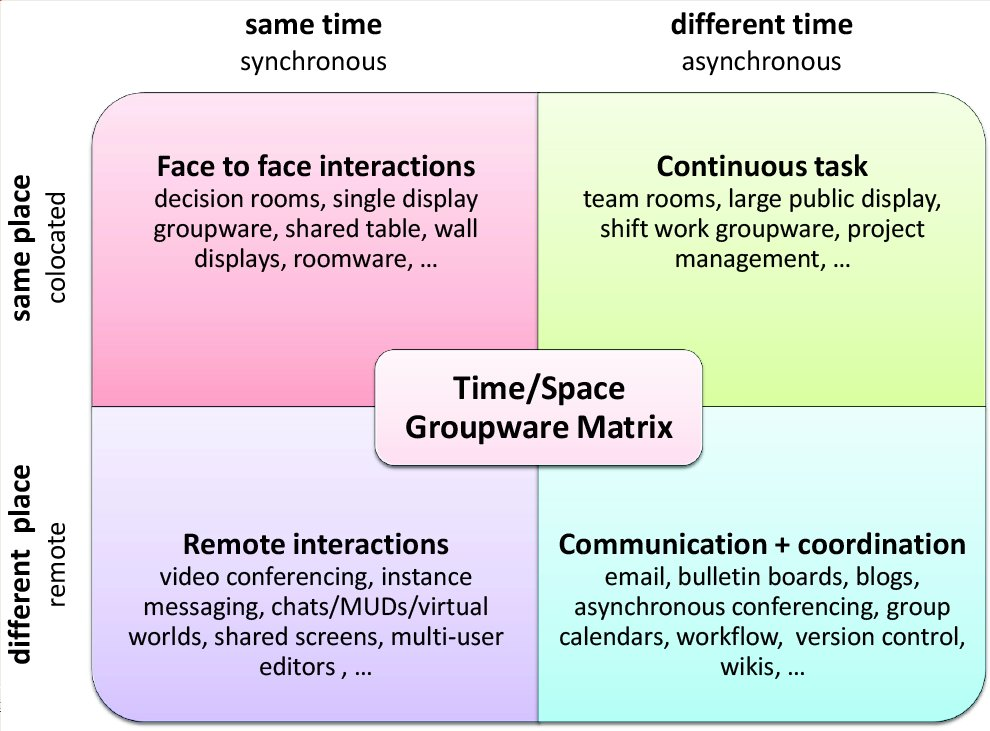
\includegraphics[scale=0.3]{img/cscw-matrix}
  \end{figure}
\end{frame}

\section{Instrumente colaborative}

\begin{frame}{Wikis}
  \begin{itemize}
    \item editare de conținut web
    \item sintaxă simplă
    \item generare rapidă de conținut
    \item colaborare facilă
    \item accent pe structură și conținut, mai puțin pe formă
    \item documentație, tutoriale, informare, proceduri
    \item MediaWiki, DokuWiki, TWiki, TikiWiki, MoinMoin, PmWiki
    \item \texttt{http://www.wikimatrix.org/}
  \end{itemize}
\end{frame}

\begin{frame}{Online Docs}
  \begin{itemize}
    \item colaborare în timp real
    \item integrare cu suite Office ``offline'' (upload, download)
    \item documente interne
    \item slide-uri, spreadsheets
    \item Google Docs, Microsoft Office Live, Oracle Cloud Office
  \end{itemize}
\end{frame}

\begin{frame}{VCS/SCM}
  \begin{itemize}
    \item Version Control System, Revizion Control System
    \item Source Code Management
    \item repository pentru cod
    \item colaborare între dezvoltatori
    \item commit-uri, ierarhie de commit-uri, istoric de modificări
    \item Git, Subversion, Perforce, Mercurial, Darcs, Bazaar
  \end{itemize}
\end{frame}

\begin{frame}{Mailing Lists/Forums/IRC/Usenet}
  \begin{itemize}
    \item discuții, întrebări, opinii, propuneri
    \item asincrone: liste de discuție, forumuri, Usenet, Google Groups
    \item sincrone: IRC, chat, video chat
    \item clienți de e-mail, clienți web, clienți IRC
  \end{itemize}
\end{frame}

\begin{frame}{Blogging}
  \begin{itemize}
    \item informare, tutoriale, comentarii
    \item asincrone
    \item în general folosite ca social software
  \end{itemize}
\end{frame}

\begin{frame}{File syncing/sharing}
  \begin{itemize}
    \item sincronizare/partajare a datelor
    \item sisteme de file-sharing
    \item rsync, Dropbox
  \end{itemize}
\end{frame}

\begin{frame}{DMS}
  \begin{itemize}
    \item Document Management System
    \item de obicei pentru instituții/companii
    \item colaborare, versionare, căutare, securitate, metadate
    \item folosit pentru documente digitale (scrise sau scanate)
    \item KnowledgeTree, Archivista, Alfresco
  \end{itemize}
\end{frame}

\begin{frame}{Calendaring}
  \begin{itemize}
    \item întâlniri, evenimente, task-uri
    \item invitații
    \item partajarea calendarului
    \item servere de calendaring (Open Calendar Server, Microsoft Exchange,
    Bedework)
    \item soluții online (Google Calendar)
  \end{itemize}
\end{frame}

\begin{frame}{LDAP/AD}
  \begin{itemize}
    \item Lightweight Directory Access Protocol / Active Directory
    \item stocarea informației într-un format de directoare (arbore):
    informații despre utilizatori, sisteme, contacte etc.
    \item folosit pentru autentificare unică
    \item OpenLDAP, Microsoft Active Directory
  \end{itemize}
\end{frame}

\begin{frame}{Groupware}
  \begin{itemize}
    \item soluție integrată
    \item e-mail (+ calendar, groups), ToDo/Tasks, Project Management
    \item eGroupWare, Horde Groupware, Kolab, Zimbra, Tiki Wiki
    \item clienți: PIM -- Personal Information Manager (Evolution, Kontact,
    Thunderbird/Lightning, Microsoft Outlook)
  \end{itemize}
\end{frame}

\begin{frame}{Software Project Management}
  \begin{itemize}
    \item soluție integrată
    \item wiki, ticket/issue trackers, repository, autentificare
    \item plugin-uri
    \item instalabile: Trac, Redmine, Launchpad, JIRA
    \item hosted: SourceForge, Google Code, CodePlex
  \end{itemize}
\end{frame}

\section{DokuWiki}

\begin{frame}{DokuWiki}
  \begin{itemize}
    \item \texttt{http://www.dokuwiki.org/}
    \item file-based (nu necesită baze de date)
    \item PHP
    \item versiune stabilă o dată la 
    \item plugin-uri
    \item access control list
    \item util pentru organizații și companii mici
  \end{itemize}
\end{frame}

\begin{frame}{De ce DokuWiki?}
  \begin{itemize}
    \item ușor de instalat și configurat (nu necesită bază de date)
    \item perfect (zic eu) pentru ``personal use'' sau echipe de oameni
    \item namespace-uri: organizarea ierarhică a informației
    \item indexarea namespace-urilor (afișarea conținutului)
    \item ușor personalizabil (template-uri, appearance)
    \item peste 750 de pluginuri
    \item gestiunea grupurilor
    \item interfață simplă și ușor de folosit
    \item interfață de administrare facilă
    \item geek mode on: fișierele sunt păstrate ``plain text'' $\rightarrow$ pot
    fi editate cu Vi :-P
    \item feeds/autentificare/comunitate/open-source
    \item e cool și hip: cel mai vizualizat pe WikiMatrix
  \end{itemize}
\end{frame}

\begin{frame}{Când folosim DokuWiki?}
  \begin{itemize}
    \item uz personal: am informații, tutoriale, pe care vreau să le public
    \item colaborare în cadrul unei echipe
    \item publicare informații utile ce pot fi completate colaborativ
    \item scopuri educaționale
    \item content management system facil de editat
  \end{itemize}
\end{frame}

\begin{frame}{Instalare și configurare}
  \begin{itemize}
    \item se descarcă \texttt{http://www.splitbrain.org/projects/dokuwiki}
    \item se dezarhivează
    \item se accesează pagina de instalare
    \item GO!
    \item se instalează plugin-uri
    \item se urmărește acest tutorial:
      \begin{itemize}
        \item \url{http://swarm.cs.pub.ro/~razvan/dokuwiki/tutorials/dokuwiki}
      \end{itemize}
  \end{itemize}
\end{frame}

\begin{frame}{Cum se folosește?}
  \begin{itemize}
    \item autentificare
    \item se parcurg namespace-urile sau se caută informație
    \item se folosește edit la nivel de pagină sau secțiune
      \begin{itemize}
        \item http://www.dokuwiki.org/syntax
        \item se poate folosi plugin de Creole
      \end{itemize}
    \item se folosesc feed-uri RSS/Atom pentru urmărirea schimbărilor
    \item crearea unei pagini se efectuează prin căutarea acesteia și apoi
    folosirea butonului \texttt{Create Page}
    \item ștergerea unei pagini se realizează prin ștergerea conținutul
    acesteia
  \end{itemize}
\end{frame}

\begin{frame}{Tips}
  \begin{itemize}
    \item folosiți feed-uri RSS/Atom
    \item faceți informația accesibilă publicului, oferiți drept de editare
    (dacă apar probleme, puteți observa în feed și face revert)
    \item folosiți pluginul indexmenu
    \item vedeți ce plugin-uri vi se par interesante
    \item folosiți o temă/template care să vă placă
    \item geek mode on: urmăriți conținutul \texttt{\$DW\_ROOT/conf/} --
    that's where the juicy stuff happens
    \item spread the word :-)
  \end{itemize}
\end{frame}

\section{Git}

\begin{frame}{Git}
  \begin{itemize}
    \item Wikipedia dixit: \textit{Git is mild profanity with origins in
    British English for a silly, incompetent, stupid, annoying, senile elderly
    or childish person. It is usually an insult, more severe than twit or
    idiot but less severe than wanker or arsehole.}
      \begin{itemize}
        \item
        \url{https://git.wiki.kernel.org/index.php/GitFaq\#Why_the_.27git.27_name.3F}
      \end{itemize}
    \item Linus Torvalds, Junio Hamano
    \item distributed VCS
    \item accent pe viteză
    \item \url{http://git-scm.com/}
    \item folosit de Linux, Gnome, KDE, GNOME, Android, X.org etc.
  \end{itemize}
\end{frame}

\begin{frame}{De ce Git?}
  \begin{itemize}
    \item distribuit: ai o copie locală a întregului arbore
    \item poți face commit-uri doar locale
      \begin{itemize}
        \item repository-uri locale
        \item fără legătură la Internet
      \end{itemize}
    \item gestiune facilă de branch-uri noi
    \item număr mare de opțiuni
    \item gamă largă de aplicații adiacente; integrare cu alte componente
    \item comunitate activă
    \item site-uri de suport, hosting, tutoriale
    \item everybody's using it
    \item setup facil: \texttt{git init --bare} $\rightarrow$ you're mostly done
  \end{itemize}
\end{frame}

\begin{frame}{Când folosim Git?}
  \begin{itemize}
    \item lucru la proiecte software de orice fel: publice, private, mari,
    mici, cu număr mare dezvoltatori, ierarhie de dezvoltatori, submodule,
    teme de casă
    \item lucru pe fișiere text (LaTeX)
    \item publicarea codului tău (share with the others)
    \item lucru la proiecte personale, pe sistemul local (pentru versionare
    locală -- teme de casă)
    \item pentru versionare locală a unor fișiere text (fișiere de configurare
    \texttt{/etc/apache2/})
    \item când vrei să publici automat informație din repository (hook-uri)
  \end{itemize}
\end{frame}

\begin{frame}{Instalare și configurare}
  \begin{itemize}
    \item \texttt{apt-get install git}
    \item pentru server se poate folosi
      \begin{itemize}
        \item SSH, git-daemon, server HTTP
        \item gitolite
        \item hosted: GitHub, Gitorious
      \end{itemize}
    \item \texttt{git config --global user.name "Razvan Deaconescu"}
    \item \texttt{git config --global user.name "razvan@rosedu.org"}
    \item \texttt{git config --global color.ui auto}
  \end{itemize}
\end{frame}

\begin{frame}{Cum se foloește?}
  \begin{itemize}
    \item \texttt{http://gitimmersion.com/}
    \item \texttt{http://www.gitready.com/}
    \item dacă există repository-ul (doar client)
      \begin{itemize}
        \item \texttt{git clone URL}
        \item simplificat: modificări, \texttt{git add}, \texttt{git commit},
        \texttt{git pull}, \texttt{git push}
      \end{itemize}
    \item dacă nu există
      \begin{itemize}
        \item creare (pe server) \texttt{git init --bare}
        \item populare repository (pe client)
          \item \texttt{git init .}
          \item \texttt{git add . \&\& git commit -m 'initial commit'}
          \item \texttt{git remote add origin URL}
          \item \texttt{git push origin master}
        \item utilizare (pe client) (ca mai sus)
      \end{itemize}
  \end{itemize}
\end{frame}

\begin{frame}{Tips}
  \begin{itemize}
    \item configurați username și e-mail înainte de toate
    \item folosiți GitHub sau Gitorious pentru proiecte generale (personale
    sau de echipă)
    \item publicați-vă codul sursă, solicitați feedback
    \item faceți commit-uri mici (do one thing)
    \item folosiți Git pentru repository-uri locale
    \item folosiți aplicații asociate: gitk, git-gui, tig, gitweb, gitolite
    \item documentați-vă constant; sunt feature-uri care vă pot fi util dar pe
    care nu le cunoașteți
    \item folosiți timpul prezent în commit-uri
    \item folosiți branch-uri
    \item folosiți \texttt{.gitignore} pentru a selecta fișierele dorite
    \item \textbf{nu} comiteți fișiere binare
    \item geek mode on: folosiți hook-uri pentru notificări sau pentru a
    publica automat conținut
  \end{itemize}
\end{frame}

\section{Redmine}

\begin{frame}{Redmine}
  \begin{itemize}
    \item open source web-based software project management
    \item wiki, issue tracker, document management, time tracking, repository
    integration, forums, calendar, Gantt chart
    \item subproiecte
    \item roluri
    \item personalizare
    \item plugin-uri
    \item Ruby on Rails
    \item \url{http://www.redmine.org/}
  \end{itemize}
\end{frame}

\begin{frame}{De ce Redmine?}
  \begin{itemize}
    \item integrarea componentelor
    \item gestiune facilă și integrată a mai multor proiecte: creare proiect +
    delegare către manager
    \item roluri pentru utilizatori
    \item suport pentru un număr variat de soluții de versionare
    \item personalizarea instanței Redmine și a proiectelor aferente
    \item notificare personalizată
    \item suport LDAP
    \item issue tracking, custom issue queries
    \item plugin-uri
    \item comunitate și suport
  \end{itemize}
\end{frame}

\begin{frame}{Când folosim Redmine?}
  \begin{itemize}
    \item proiecte software de toate tipurile
    \item gestiunea unei echipe
  \end{itemize}
\end{frame}

\begin{frame}{Instalare și configurare}
  \begin{itemize}
    \item \texttt{apt-get install redmine}
    \item se alege tipul de baze de date folosit
    \item se integrează în Apache (\texttt{mod\_passenger} sau
    \texttt{mod\_fcgid})
    \item se realizează autentificarea și se configurează elementele
    importante
      \begin{itemize}
        \item forme de autentificare
        \item forme de notificare
        \item roluri
        \item enumerări: stări ale unui issue, tipuri de documente etc.
      \end{itemize}
    \item se creează proiecte și utilizatori
    \item se adaugă un manager unui proiect și se deleagă configurarea
    proiectului
  \end{itemize}
\end{frame}

\begin{frame}{Cum se foloește?}
  \begin{itemize}
    \item interfață web: autentificare și acțiuni
    \item editare wiki
    \item creare/actualizare issue-uri
    \item upload documente/fișiere
    \item browser pentru repository
    \item folosire forumuri
  \end{itemize}
\end{frame}

\begin{frame}{Tips}
  \begin{itemize}
    \item folosire feed-uri: activități și/sau issue-uri
    \item un proiect în Redmine per activitate/proiect; se pot crea ușor
    proiect/subproiecte
    \item folosire issue-uri pentru planificare, bug-uri, task-uri: sunt
    persistente, nu se uită
    \item folosire custom issue queries pentru vizualizare issue-uri
    \item folosire autentificare prin LDAP
    \item instalare plugin-uri utile
    \item personalizare pagină principală și opțiuni specifice contului
    (notificări primite)
  \end{itemize}
\end{frame}

\section{Concluzii}

\begin{frame}{Cuvinte cheie}
  \begin{columns}
    \begin{column}[l]{0.5\textwidth}
      \begin{itemize}
        \item TODO
      \end{itemize}
    \end{column}
    \begin{column}[l]{0.5\textwidth}
      \begin{itemize}
        \item TODO
      \end{itemize}
    \end{column}
  \end{columns}
\end{frame}

\begin{frame}{Resurse utile}
  \begin{itemize}
    \small
    \item TODO
  \end{itemize}
\end{frame}

\section{Întrebări}

\end{document}
